% This file demonstrates how to use the IEEEConf LaTeX2e macro package,
% to prepare a manuscript for proceedings on CD of the conference
% FedCSIS
%
\documentclass[conference]{IEEEtran}
%\documentclass[a4paper]{IEEEconf}

% This package serves to balance the column lengths on the last page of the document.
% please, insert \balance command in the left column of the last page
\usepackage{balance}

%% to enable \thank command
\IEEEoverridecommandlockouts 
%% The usage of the following packages is recommended
%% to insert graphics
\usepackage{graphicx}
% to typeset algorithms
%\usepackage{algorithmic}
\usepackage{algorithm}
% to typeset code fragments
\usepackage{listings}
% to make an accent \k be available
\usepackage[OT4,T1]{fontenc}
% provides various features to facilitate writing math formulas and to improve the typographical quality of their output.
\usepackage[cmex10]{amsmath}
\interdisplaylinepenalty=2500
% por urls typesetting and breaking
\usepackage{url}
% for vertical merging table cells
\usepackage{multirow}

\usepackage{filecontents}

\usepackage{color}
\usepackage{xcolor}
\usepackage{colortbl}
\definecolor{LightCyan}{rgb}{0.88,1,1}
\definecolor{BluishGray}{RGB}{226,227,231}
\definecolor{LightGray}{gray}{0.95}
\definecolor{Gray}{gray}{0.85}
\usepackage{algpseudocode,algorithmicx}
\usepackage{comment}
\newcommand*\DNA{\textsc{dna}}

\newcommand*\Let[2]{\State #1 $\gets$ #2}
\algrenewcommand\algorithmicrequire{\textbf{Input:}}
\algrenewcommand\algorithmicensure{\textbf{Output:}}
\algrenewcommand\algorithmicrequire{\textbf{Input:}}
\algrenewcommand\algorithmicensure{\textbf{Output:}}

% define environments for remarks and examples
\newtheorem{remark}{Remark}[section]
\newtheorem{example}[remark]{Example}
\newcommand{\ti}{\textit}
\newcommand{\tb}{\textbf}

\setlength{\textfloatsep}{1\baselineskip plus 0.2\baselineskip minus 0.8\baselineskip}



%
%
\title{From UML State Machine to code and back again!}
%
%
\author{
\IEEEauthorblockN{Van Cam Pham, Ansgar Radermacher, S\'{e}bastien G\'{e}rard}
\IEEEauthorblockA{
CEA-List, Laboratory of Model-Driven Engineering for Embedded Systems (LISE)\\
Gif-sur-Yvette, France\\
Email: first-name.lastname@cea.fr}
}

% conference papers do not typically use \thanks and this command
% is locked out in conference mode. If really needed, such as for
% the acknowledgment of grants, issue a \IEEEoverridecommandlockouts
% after \documentclass

% for over three affiliations, or if they all won't fit within the width
% of the page, use this alternative format:
% 
%\author{\IEEEauthorblockN{Michael Shell\IEEEauthorrefmark{1},
%Homer Simpson\IEEEauthorrefmark{2},
%James Kirk\IEEEauthorrefmark{3}, 
%Montgomery Scott\IEEEauthorrefmark{3} and
%Eldon Tyrell\IEEEauthorrefmark{4}}
%\IEEEauthorblockA{\IEEEauthorrefmark{1}School of Electrical and Computer Engineering\\
%Georgia Institute of Technology,
%Atlanta, Georgia 30332--0250\\ Email: see http://www.michaelshell.org/contact.html}
%\IEEEauthorblockA{\IEEEauthorrefmark{2}Twentieth Century Fox, Springfield, USA\\
%Email: homer@thesimpsons.com}
%\IEEEauthorblockA{\IEEEauthorrefmark{3}Starfleet Academy, San Francisco, California 96678-2391\\
%Telephone: (800) 555--1212, Fax: (888) 555--1212}
%\IEEEauthorblockA{\IEEEauthorrefmark{4}Tyrell Inc., 123 Replicant Street, Los Angeles, California 90210--4321}}





\begin{document}
\maketitle              % typeset the title of the contribution

\begin{abstract}
%The so-called model-driven engineering approach relies on two paradigms, abstraction and automation, recognized as very efficient for dealing with complexity of today system. 
%Abstraction is the ability to provide simplified and focused view of a system and requires adequate modeling language. 
%For this concern, it is clear that the Unified Modeling Language (UML) is nowadays the most used, educated, documented and tooled modeling language. 
%Even, if a graphical language such as the UML is not the silver bullet for all software related concerns, it provides hence better support than text-based solutions for some concerns such as architecture and logical behavior of application development. 
UML state machine and their visual representations are much more suitable to describe logical behaviors of system entities than any equivalent text based description such as IF-THEN-ELSE or SWITH-CASE constructions. Although many industrial tools and research prototypes can generate executable code from such graphical language, generated code could be manually modified by programmers. 
After code modifications, round-trip engineering is needed to make the model and code consistent, which is a critical aspect to meet quality and performance constraint required from project manager today. Unfortunately, current UML tools only support structural concepts for round-trip engineering such as those available from class diagrams. In this paper, we address the round-trip engineering of UML state-machine and its related generated code. We propose a round-trip engineering approach consisting of a forward process which generates code by using transformation patterns, and a backward process which is based on code pattern detection to update the original state machine model from the modified generated code. We implemented a prototype and conducted several experiments on different aspects of the round-trip engineering to verify the proposed approach.


%Unified Modeling Language (UML) State machine is widely used 

%Model-driven engineering (MDE) is a development methodology aiming to increase software productivity and quality by automatically generating code from higher level abstraction models. 
%A recent survey has revealed that industries are gaining the adoption of code generation into software development life-cycle. 
%Although many tools and research prototypes can generate executable code from models (e.g. Unified Modeling Language), developers, after code generation, tend to abandon models and code generators in software evolution. The reason behind is that generated code could be manually modified by developers and code modifications are not easily propagated back to models. Round-trip engineering (RTRIP) supported by many tools is needed to make the model and code consistent but most of the tools are only applicable to static diagrams such as classes. In this paper, we tackle a classical problem : from UML State Machine diagrams to code and back. We propose a RTRIP approach consisting of a forward process, which generates code, and a backward process, which updates the original state machine from the modified generated code. From the proposed approach, we implemented a prototype and conducted several experiments on different aspects of the round-trip engineering to verify the proposed approach.
\end{abstract}

\begin{comment}
\section{Figures and Tables}
To insert a figure you are encouraged to use the  \verb|graphicx| package. Please, include this package in the preamble with the option \verb|dvips|:
\begin{verbatim}
\usepackage[dvips]{graphicx}
\end{verbatim}
Figures in the \verb|eps| format should be inserted in the \verb|figure| environment, as follows:
\begin{verbatim}
\begin{figure}[tbp]
\centering
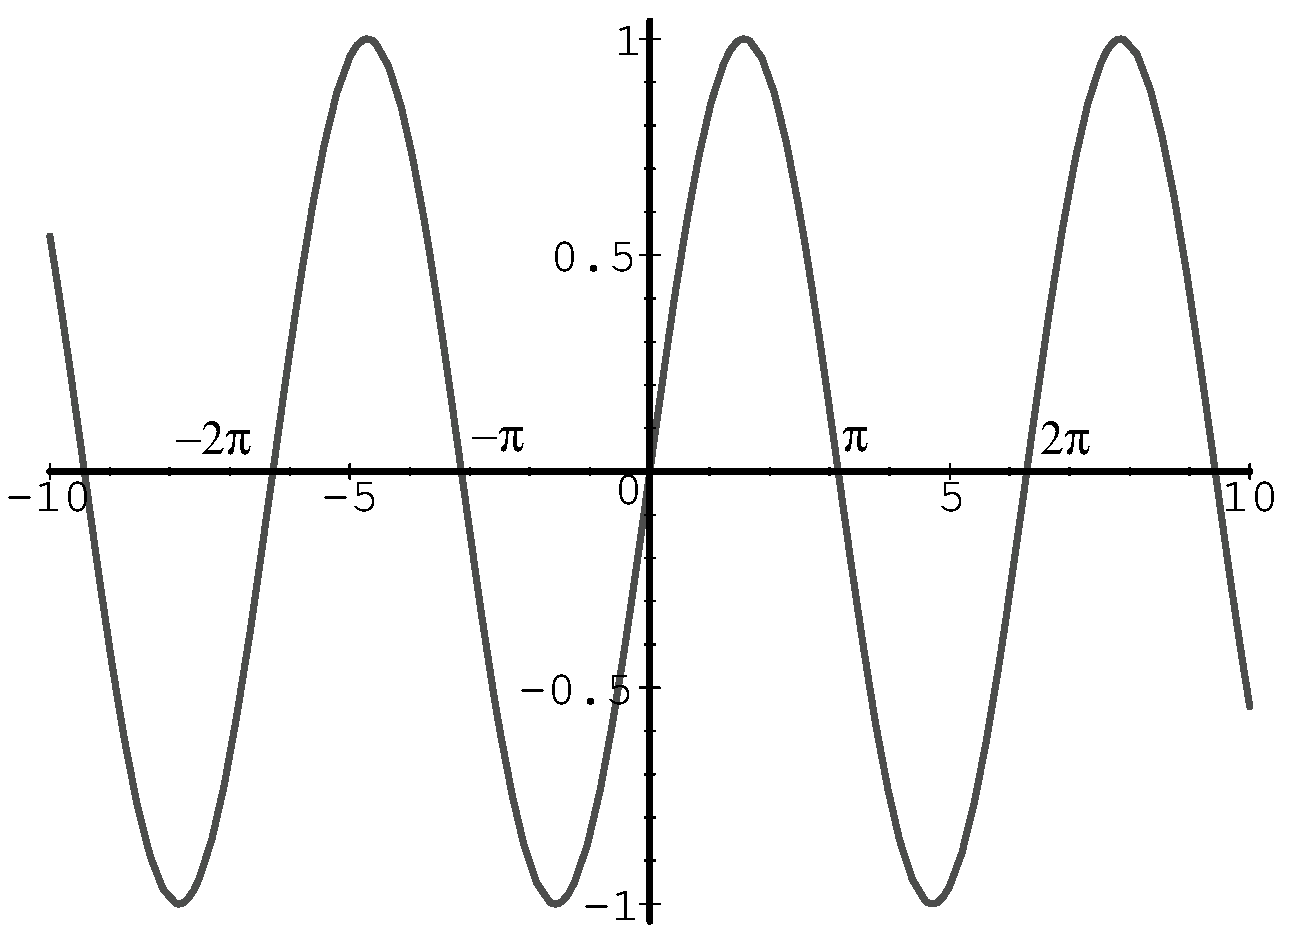
\includegraphics[width=0.75\hsize]
     {test.eps}
\caption{Sinusoid}
\end{figure}
\end{verbatim}
%
\end{comment}

%Test the change

%Some terms to find, define, and keep coherent:
%- Developer
%- The developer who uses models is called... (e.g. software architect modeler? doesn't mean anything)
%- The developer who uses code is called... (e.g. programmer)
%- Our method is for... called... (e.g. method for model code synchronization, method for architect/programmer collaboration, etc...)
%- Model is...
%- Code is...
%- Gap or difference ?
%- Background or practice or habits or profiles ? Maybe keep profile and choose one of the other?


\section{Introduction}
\label{sec:introduction}
The so-called Model-Driven Engineering (MDE) approach relies on two paradigms, abstraction and automation \cite{Mussbacher2014}. It is recognized as very efficient for dealing with complexity of today system. 
%Abstraction is the ability to provide simplified and focused view of a system and requires adequate modeling language. 
%Unified Modeling Language (UML) \cite{Specification2007} is nowadays the most used, educated, and documented modeling language. 
%Even, if a graphical language such as Unified Modeling Language (UML) \cite{Specification2007} is not the silver bullet for all software related concerns, it provides hence better support than text-based solutions for some concerns such as architecture and logical behavior of application development. 
Abstraction provides simplified and focused views of a system and requires adequate graphical modeling languages such as Unified Modeling Language (UML). Even, if the latter is not the silver bullet for all software related concerns, it provides better support than text-based solutions for some concerns such as architecture and logical behavior of application development. UML state machines (USMs) and their visual representations are much more suitable to describe logical behaviors of system entities than any equivalent text based descriptions. The gap from USMs to system implementation is reduced by the ability of automatically generating code from USMs  \cite{Booch1998, Douglass1999,Shalyto2006,Douglass1999}. 

Ideally, a full model-centric approach is preferred by MDE community due to its advantages \cite{Selic2012}. However, in industrial practice, there is significant reticence \cite{Hutchinson:2011:MEP:1985793.1985882} to adopt it.
On one hand, programmers prefer to
use the more familiar textual programming language. 
On the other hand, software architects, working at higher levels
of abstraction, tend to favor the use of models, and therefore
prefer graphical languages for describing the architecture of
the system.
%However, on the one hand, maintaining code generated from existing approaches is non-trivial. On the other hand our observation is that it is very difficult to come up with formalizations that yield such elegant code generation solutions \cite{6032552}. In other words, generated code must be manually modified to build fully operational applications. 
%On one hand there are traditional developers who prefer to implement the system by writing code, while on the other hand there are developers who prefer to use entirely models for the design and implementation of the system. 
The code modified by programmers and the model are then inconsistent. Round-trip engineering (RTE) \cite{Hettel2008} is proposed to synchronize different software artifacts, model and code in this case \cite{Sendall}. RTE enables actors (software architect and programmers) to freely move between different representations \cite{Sendall} and stay efficient with their favorite working environment. 

%After code modifications, round-trip engineering (RTE) is needed to make the model and code consistent, which is a critical aspect to meet quality and performance constraint required from project managers today. 
Unfortunately, current industrial tools such as for instance Enterprise Architect \cite{sparxsystems_enterprise_2014} and IBM Rhapsody\cite{ibm_rhapsody} only support structural concepts for RTE such as those available from class diagrams and code. Compared to RTE of class diagrams and code, RTE of USMs and code is non-trivial. It requires a semantical analysis of the source code, code pattern detection and mapping patterns into USM elements. 
This is a hard task, since mainstream programming languages such as C++ and JAVA do not have a trivial mapping between USM elements and source code statements.

For software development, one may wonder whether this RTE is doable. That is, why do the industrial tools not support the propagation of source code modifications back to original state machines? Several possible reasons to this lack are (1) the gap between USMs and code, (2) not every source code modification can be reverse engineered back to the original model, and (3) the penalty of using transformation patterns facilitating the reverse engineering that may not be the most efficient (e.g. a slightly larger memory overhead). 
%in the mind of these tools' vendors, users always make changes to models rather than to code. Generated code, in these tools, is therefore not supposed to be changed directly.  
 
%In this paper, we address the RTE of UML State Machine diagrams and its related generated code. We propose a RTE approach consisting of a forward process which generates code by using transformation patterns, and a backward process which is based on code pattern detection to update the original state machine model from the modified generated code. From the proposed approach, we implemented a prototype and conducted several experiments on different aspects of the round-trip engineering to verify the proposed approach. 



%Model-driven engineering (MDE) is a development methodology aiming to increase software productivity and quality by allowing different stakeholders to contribute to the system description \cite{Mussbacher2014}. MDE considers models as first-class artifacts and generates code from higher abstraction level models. Recent survey \cite{1030} has revealed that industries are gaining the adoption of code generation into software development life-cycle. Although many tools and research prototypes can generate executable code from models, generated code could be manually modified by programmers, e.g. skeleton code generated from UML \cite{Specification2007} class diagrams. Models and the generated code are therefore out of synchronization. Round-trip engineering \cite{Aßmann200333, Hettel2008, E-ESE-120044648} (RTE) is proposed to keep the artifacts synchronized.

%RTE supports synchronizing different software artifacts, model and code in this case, and thus enabling actors (software architect and programmers) to freely move between different representations \cite{Sendall}. Tools such as for instance Enterprise Architect \cite{sparxsystems_enterprise_2014}, Visual Paradigm \cite{visual}, and AndroMDA \cite{_andromda_} provide RTE but most of them are only applicable for system structure models such as class diagrams.  

%This study addresses the RTE of UML State Machine (SM) and object-oriented programming languages such as C++ and JAVA. SM is widely used in practice for modeling the behavior of complex systems, notably reactive, real-time embedded systems. There are several approaches to generating source code from state machines or state charts such as nested switch/if statements \cite{Booch1998}, state-event-table \cite{Douglass1999, Duby2001}, and state pattern \cite{Allegrini2002,Shalyto2006,Douglass1999}. Unfortunately, the generated code from these approaches is very difficult for programmers to maintain without an appropriate supporting tool. RTE is impossible in these approaches even with very small changes such as changing transition targets or actions made to code. The reason behind this impossibility is that, in mainstream programming languages such as C++, JAVA, (1) there are not equivalents between SMs and source code statements and (2) the code generation pattern of these approaches has not been chosen with RTE in mind.

%This paper addresses the RTE of UML state-machines and object-oriented programming languages such as C++ and JAVA. The forward  engineering of the approach takes as input a state-machine and executes two transformations. The first is UML to UML by utilizing several transformation patterns such as the double-dispatch approach presented in \cite{spinke_object-oriented_2013} and the second is a generation of code from the transformed UML. Traceability information is stored, during the transformations. In the backward direction, a verification is executed by the code pattern detection to verify the correctness of the code before the backward process taking as input the modified generated code, the UML classes, the original state-machine and mapping information together merges changes from code to the state-machine. We implemented a prototype supporting RTE of state-machine and C++ code, and conducted several experiments on different aspects of the RTE to verify the proposed approach. To the best of our knowledge, our implementation is the first tool supporting RTE of SM and code. 
%The prototype also improves the collaboration between MDE developers and traditional programmers in developing reactive complex embedded systems.

This paper addresses the RTE of USMs and object-oriented programming languages such as C++ and JAVA. The main idea is to utilize transformation patterns from USMs to source code that aggregates code segments associated with a USM element into source code methods/classes rather than scatters these segments in different places. Therefore, the reverse direction of the RTE can easily statically analyze the generated code by using code pattern detection and maps the code segments back to USM elements. Specifically, in the forward direction, we extend the double dispatch pattern presented in \cite{spinke_object-oriented_2013}. Traceability information is stored during the transformations. We implemented a prototype supporting RTE of state-machine and C++ code, and conducted several experiments on different aspects of the RTE to verify the proposed approach. To the best of our knowledge, our implementation is the first tool supporting RTE of SM and code. 

To sum up, our contribution is as followings:
\begin{itemize}
  \item An approach to round-tripping USMs and object-oriented code.
  \item A first tooling prototype supporting RTE of USMs and C++ code.
  \item An evaluation of the proposed approach including:
  \begin{itemize}
 	 \item An automatic evaluation of the proposed RTE approach with the prototype.% including 300 random generated SM models containing 80 states, more than 230 transitions, more than 250 actions and around 180 events for each.
  	 %\item A complexity analysis of the approach and performance evaluation.
  	 \item A comparison and collaboration of two software development practices including working at the model level and at the code level.
  	 \item A lightweight evaluation of the semantic conformance of the runtime execution of generated code.
  	\end{itemize}
\end{itemize}

The remaining of this paper is organized as follows: Our proposed approach is detailed in Section \ref{sec:approach}. The implementation of the prototype is described in Section \ref{sec:implementation}. Section \ref{sec:experiments} reports our results of experimenting with the implementation and our approach. Section \ref{sec:related_works} shows related work. The conclusion and future work are presented in Section \ref{sec:conclusion}.


\section{Approach}
\noindent
\tb{State}

\section{implementation}
\label{sec:implementation}
The proposed approach is implemented in a prototype existing as an extension of the Papyrus modeler [4]. Each state machine is created by using a state machine diagram and contained in a component. Low-level processing of state machine actions is directly embedded by a block of code written specific programming languages such as C++/JAVA in the state machine. C++ code is generated by the prototype but other object-oriented languages are easily generated. The code generation consists of transforming the state machine to UML classes and eventually to code by a code generator following the proposed approach. In the reverse direction, code pattern detection is implemented as described in the previous section to verify state machine semantics in code. If the generated code is modified, two options are supported by the prototype interface to make the state machine and code consistent again. One is to create a new state machine from the modified code in the same Eclipse project and the other one is to update the original state machine by providing as input the intermediate model and the state machine in a dialog.
\section{Experiments}
\label{sec:experiments}
In order to evaluate the proposed approach, we answer three questions stated as followings. 

\tb{RQ1}: A state machine \ti{sm} is used for generating code. The generated code is reversed by the backward transformation to produce another state machine \ti{sm'}. Are \ti{sm} and \ti{sm'} identical? In other words: whether the code generated from USMs model can be used for reconstructing the original model. This question is related to the \ti{GETPUT} law defined in \cite{foster_combinators_2007}.

\tb{RQ2}: \tb{RQ1} is related to the static aspect of generated code. \tb{RQ2} targets to the dynamic aspect. In other words, whether the runtime execution of code generated from USMs by the generator is semantic-conformant \cite{OMG2015}?

\tb{RQ3}: RTE allows developers to freely move between and modify model and code. Specifically, in software development projects, some traditional programmers might want to practice with code in a traditional way and some MDE developers may prefer working with models. What is the development/maintenance cost comparison between the two practices by comparing the number of steps needed to do equivalent actions?

This section reports our experiments targeting the three questions. Three types of experiments are conducted and presented in Subsections \ref{subsec:exp1}, \ref{subsec:exp2}, and \ref{subsec:cost}, respectively. 

\begin{comment}
\begin{figure}
\centering
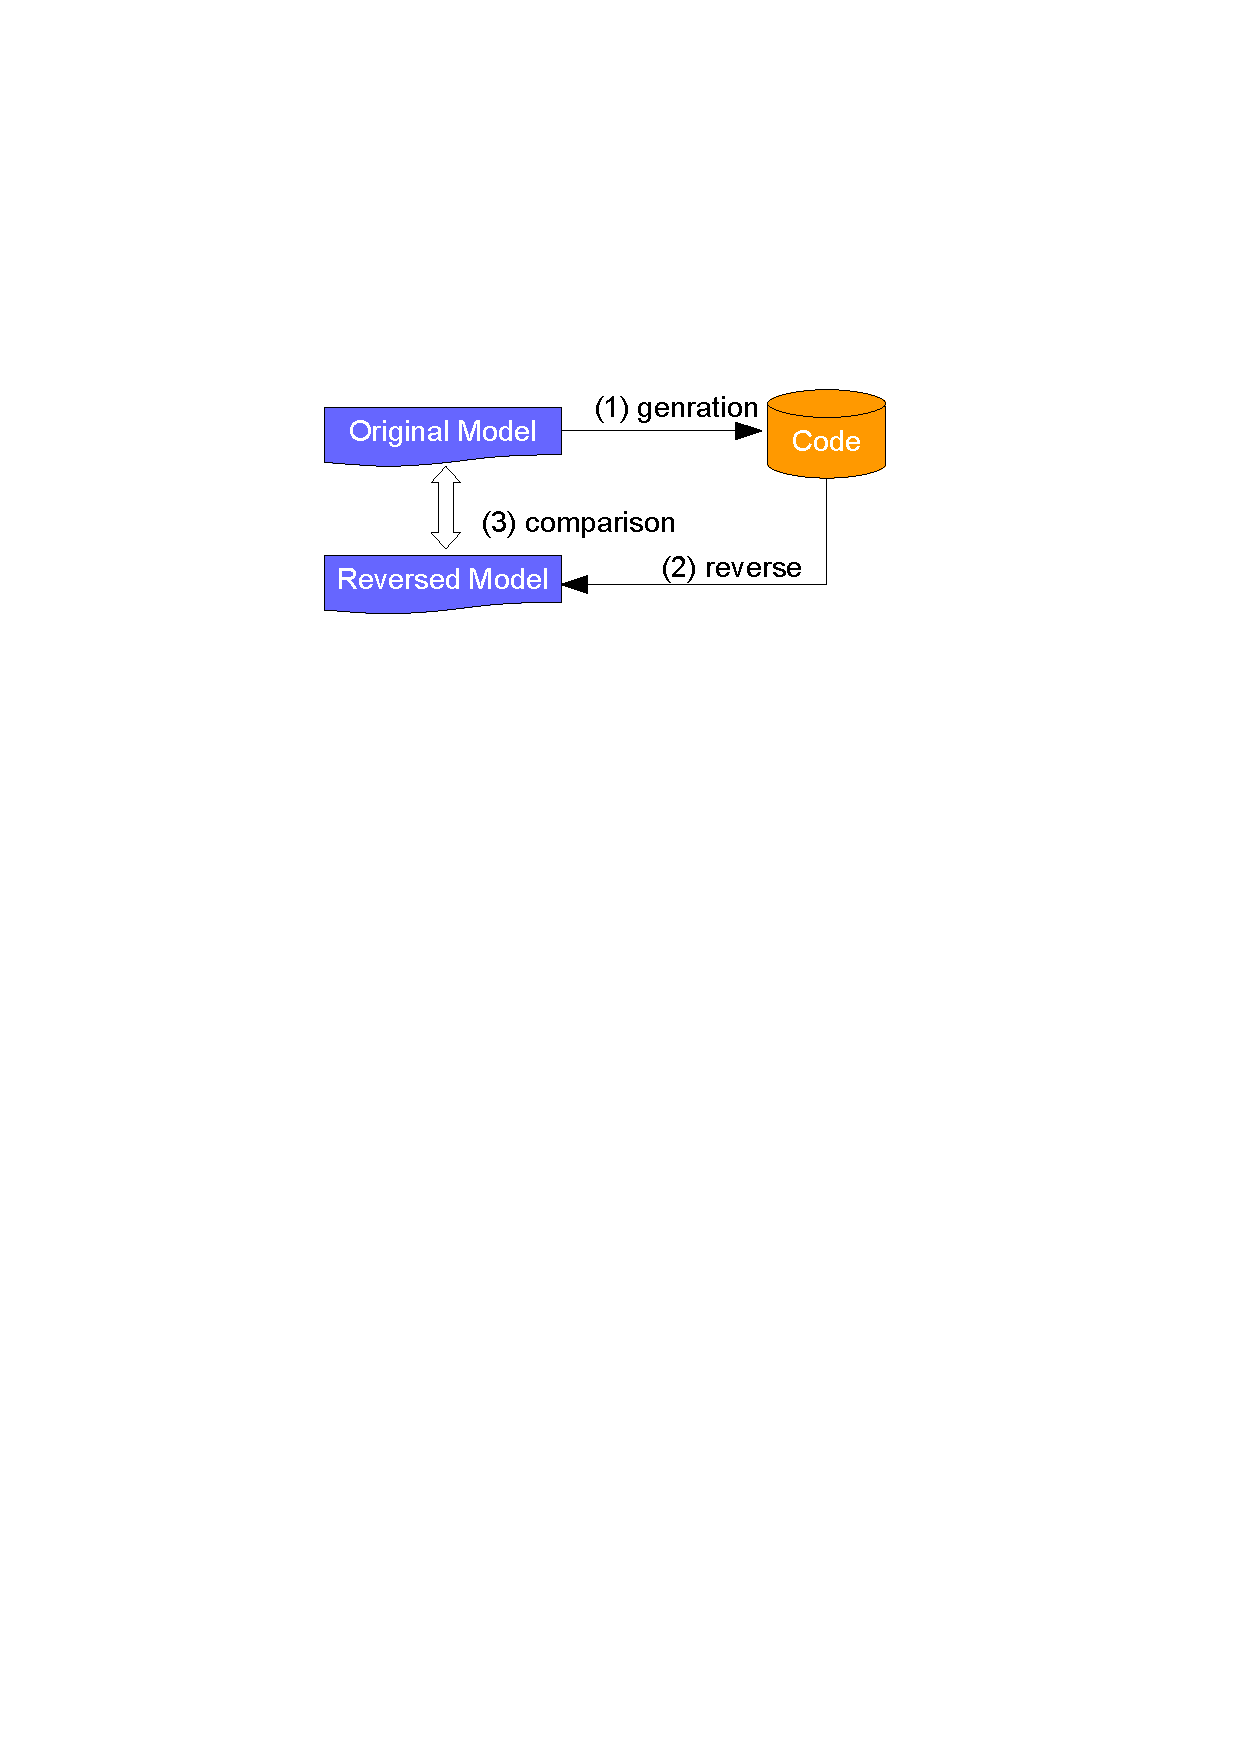
\includegraphics[clip, trim=5.5cm 19cm 5.5cm 6cm, width=0.3\textwidth]{figures/strategy1}
\caption{Evaluation methodology to answer RQ1} 
\label{fig:strategy1}
\end{figure}

\begin{figure}
\centering
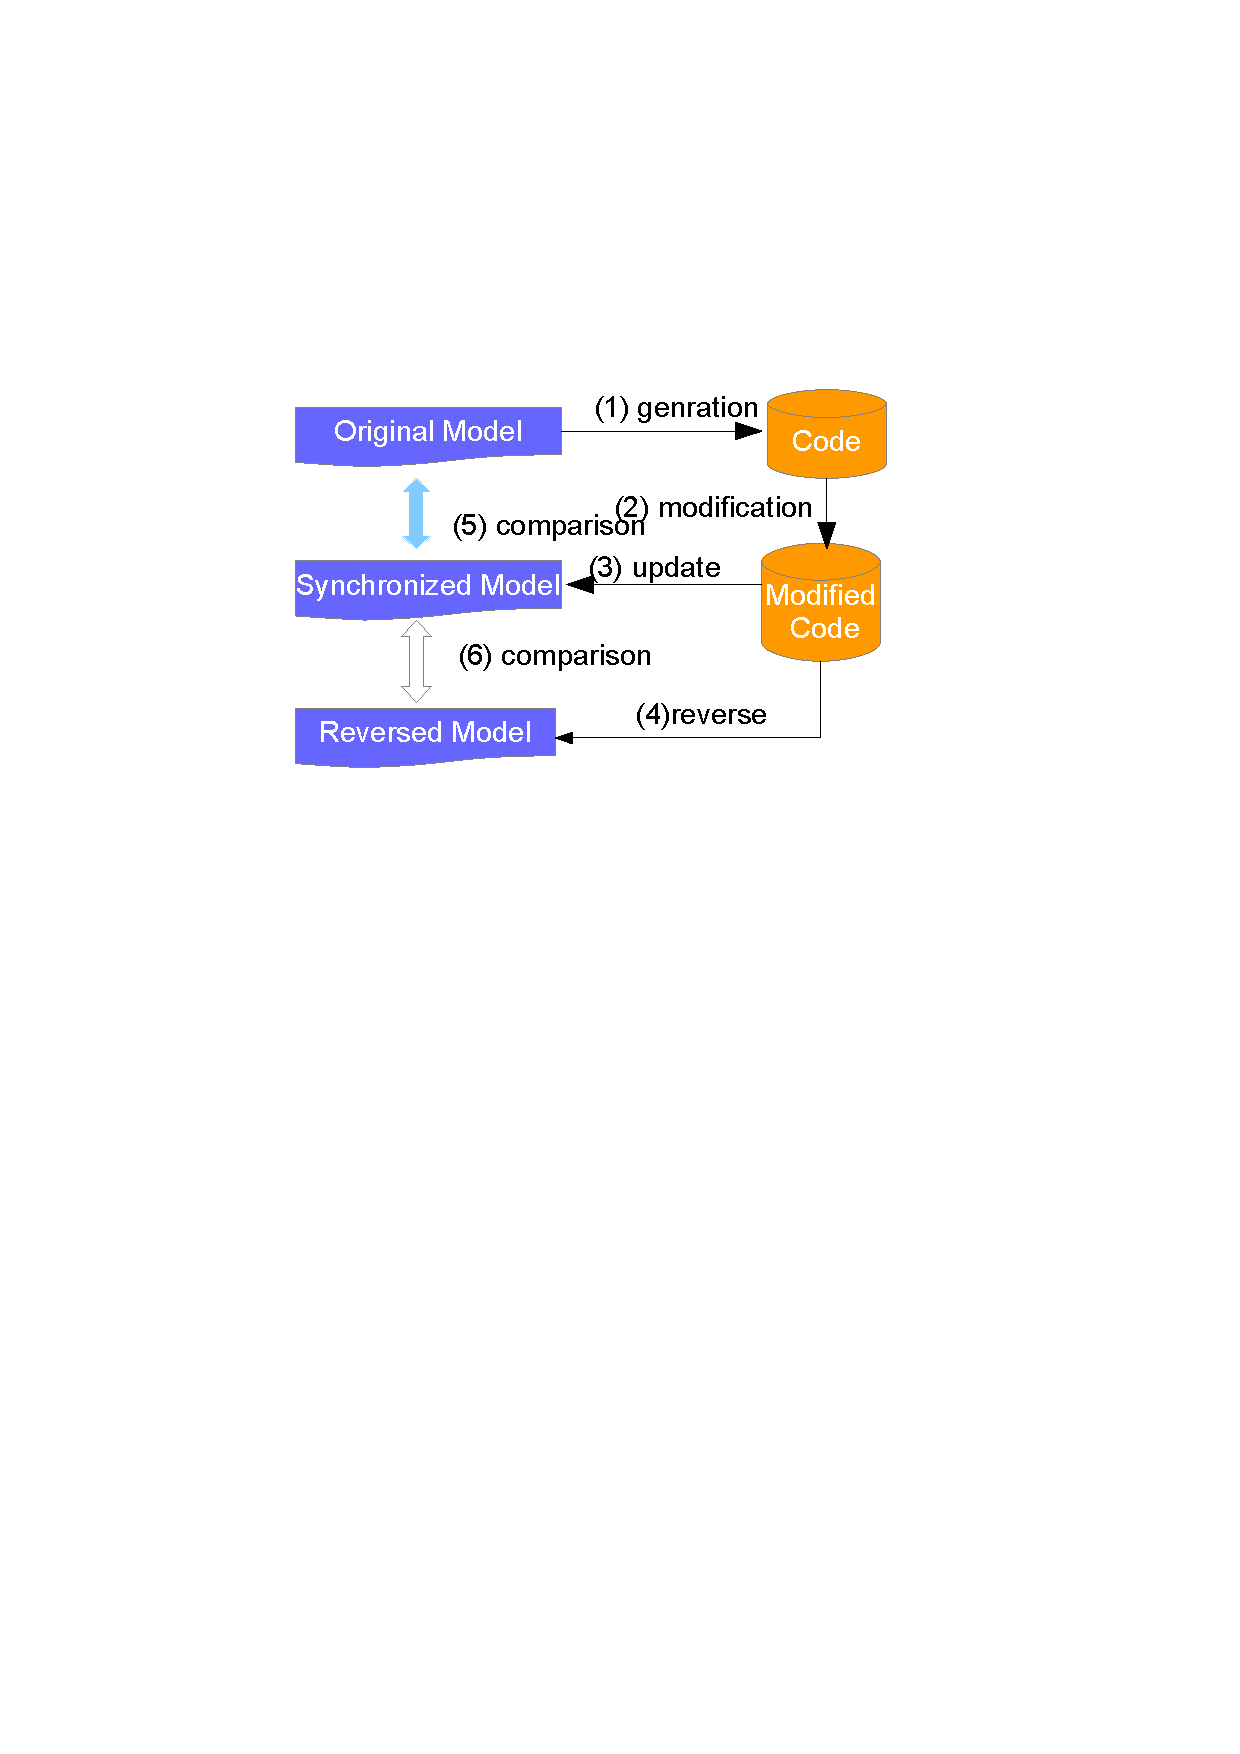
\includegraphics[clip, trim=4.5cm 16.5cm 5.5cm 6.5cm, width=0.3\textwidth]{figures/strategy2}
\caption{Evaluation methodology to answer RQ2} 
\label{fig:strategy2}
\end{figure}
\end{comment}

%Furthermore, in software development projects, some traditional programmers might want to practice with code in a traditional way and some MDE developers may prefer working with models. Therefore, it is necessary to compare the development/maintenance cost between the two practices by comparing the number of steps needed to do the same action. 


\subsection{Reversing generated code}
\label{subsec:exp1}


\begin{figure}
	\centering
	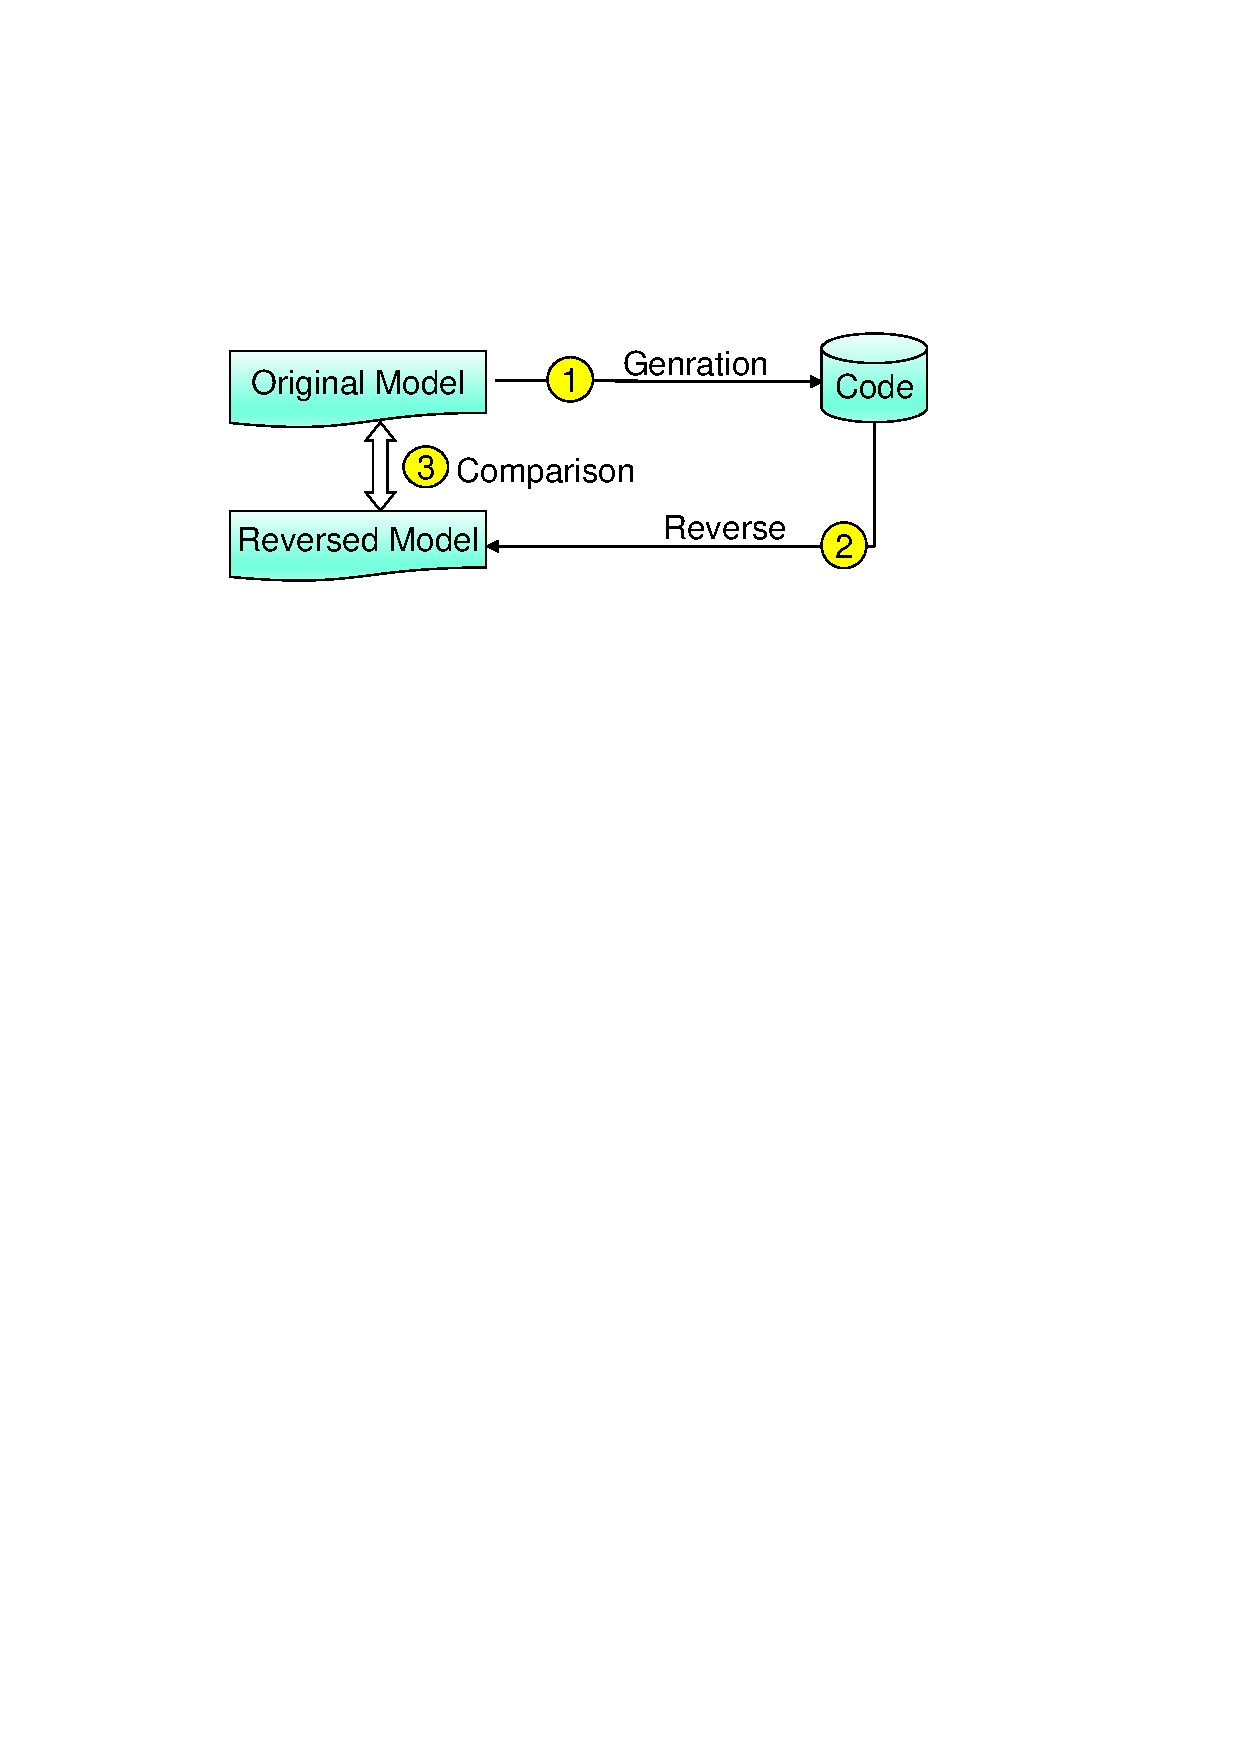
\includegraphics[clip, trim=3.3cm 19.8cm 5.2cm 5.6cm, width=0.6\columnwidth]{figures/EvaluationStrategyBoth}
	\caption{Evaluation methodology to answer RQ1} 
	\label{fig:EvaluationStrategyBoth}
\end{figure}

This experiment is targeting \tb{RQ1}. 
Fig. \ref{fig:EvaluationStrategyBoth} shows the experimental methodology to answer \tb{RQ1}. 
The procedure for this experiment, for each original UML model containing a state machine, consists of 3 steps: (1) code is generated from an \tb{original model}, (2) the generated code is reversed to a \tb{reversed model}, and (3) the latter is then compared to the \tb{original state machine}.% by using information of USM such as the numbers of states and transitions. 

Random models containing hierarchical state machines are automatically generated by a configurable model generator. 
The generator can be configured to generate a desired average number of states and transitions. 
For each model, a context class and its behavior described by a USM are generated. Each USM contains 80 states including atomic and composite states, more than 234 transitions. The number of lines of generated C++ code for each machine is around 13500. Names of the generated states are different. An initial pseudo state and a final state are generated for each composite state and containing state machine. Other elements such as call events, time events, transition/entry/exit actions and guards are generated with a desired configuration. For each generated call event, an operation is generated in the context class which is also generated. The duration is generated for each time event. 

\begin{comment}
\begin{table}
\centering
\caption{Set-up information for model generation}
\label{table:setup}
\begin{tabular}{|l|l|}
\hline
\rowcolor{Gray}
Description                                     & Value            \\ \hline
%Number of generated states                      & 80               \\ \hline
%Number of generated transitions                 & \textgreater 234 \\ \hline
Probability of having an event for transition   & 0.8              \\ \hline
Probability of having CallEvent for transition  & 0.7              \\ \hline
Probability of having an entry/exit action for state & 0.7              \\ \hline
Probability of having a transition action and guard       & 0.7              \\ \hline
\end{tabular}
\end{table}
\end{comment}

%The set up information for the USM generation is shown in Table \ref{table:setup}. 

\begin{table}
\centering
\caption{Three of model results of generation and reverse: Abbreviations are atomic states (AS), composite states (CS), transitions (T), call events (CE), time events (TE)}
\label{table:law1-resultat}
\begin{tabular}{|l|l|l|l|l|l|l|}
\hline
\rowcolor{Gray}
Test ID & AS & CS & T & CE & TE & Is reverse correct? \\ \hline
1       & 47 & 33 & 234 & 145 & 40 & Yes                 \\ \hline
2       & 42 & 38 & 239 & 145 & 36 & Yes                 \\ \hline
%3       & 43 & 37 & 238 & Yes                 \\ \hline
..      & .. & .. & .. & .. & .. & Yes                 \\ \hline
300       & 41 & 39 &240 & 142 & 37 & Yes                 \\ \hline
\end{tabular}
\end{table}
 
 
\begin{comment}
\begin{table*}[]
\centering
\caption{MODEL RESULTS OF GENERATION AND REVERSE}
\label{table:law1-resultat}
\begin{tabular}{|l|l|l|l|l|l|l|l|l|l|l|l|l|l|}
\hline
\rowcolor{Gray}
Test ID & AS & CS & D  & T   & EA & ExA & TA  & CE  & TE & G   & I  &    & Is reverse correct? \\ \hline
1       & 47 & 33 & 8  & 234 & 53 & 50  & 149 & 145 & 40 & 147 & 34 & 25 & Yes                 \\ \hline
2       & 42 & 38 & 8  & 239 & 52 & 59  & 165 & 145 & 36 & 133 & 39 & 31 & Yes                 \\ \hline
3       & 43 & 37 & 7  & 238 & 54 & 59  & 159 & 141 & 34 & 145 & 38 & 28 & Yes                 \\ \hline
..      & .. & .. & .. & ..  & .. & ..  & ..  & ..  & .. & ..  & .. & .. & Yes                 \\ \hline
300       & 41 & 39 & 10 & 240 & 56 & 55  & 165 & 142 & 37 & 151 & 40 & 33 & Yes                 \\ \hline
\end{tabular}
\end{table*}
\end{comment}

%Table  \ref{table:law1-resultat} shows the number of each type of elements in the randomly generated model, including the comparison results, for 3 of the 200 models created by the generator. We limited ourselves to 200 models for practical reasons

Table \ref{table:law1-resultat} shows the number of several types of elements in the generated models, including the comparison results, for 3 of the 300 models created by the generator. We limited ourselves to 300 models for practical reasons. No differences were found during model comparison. The results of this experiment show that the proposed approach and the implementation can successfully do code generation from state machines and reverse. 

%\subsection{Change propagation} 
We manually created two state machines (model level): one describing Java Thread life-cycle \cite{_java_thread} and the other one representing a telephone presented in \cite{Specification2007}. For each SM code is generated. Code is then manually modified. Each modification test consists of one or several actions described in Table \ref{table:cost}. The original SM is updated by doing a backward process from the modified generated code with the presence of the intermediate and original model. The updated SM ($sm_{updated}$) is in turn compared with the SM created ($sm_{reversed}$) by the reverse engineering (see Fig. \ref{fig:EvaluationStrategyBoth}). A modification test is passed if the corresponding models $sm_{updated}$ and $sm_{reversed}$ are the same. Table \ref{table:change-propa} shows the number of test cases (Tests) applied to each model, of passed test cases (Passed tests) and the result of change propagation experiment. The table shows that our approach is able to update the original state machine following code-side modifications. 

\begin{table}
\centering
\caption{Change propagation experimental results}
\label{table:change-propa}
\begin{tabular}{|l|l|l|p{3.4cm}|}
\hline
\rowcolor{Gray}
State machine & Tests & Passed tests & Is change propagation passed? \\ \hline
Java Thread       &    20     &    20      &     Yes             \\ \hline
Telephone       &   30      &     30     &      Yes       \\ \hline
\end{tabular}
\end{table}

%\subsection{Time complexity and performance}
%We are interested in knowing which element type among state, transition and event dominates the running time of the reverse engineering in case of creating new SM from code. 
To analyze the time complexity, we consider two tasks: semantic verification and SM construction from the verification output. 
%Let us use the following parameters of the input SM used in code generation: $n_{s}$ = number of states, $n_{t}$ = number of transitions, $n_{ce}$ = number of call events, $n_{te}$ = number of time events, $n_{a}$ = number of actions and guards including entry/exit/transition actions and guards which are all implemented in the context class. 

For each state, the semantic verification consists of the following phases: (1) detecting composite/sub-state pattern, (2) loop over all methods of a state class, (3) detecting entry action pattern, (4) detecting exit action pattern, (5) detecting processing \ti{CallEvent}, (6) detecting processing \ti{TimeEvent}, and (7) detecting default state pattern. 
\begin{comment}
\begin{itemize}
  \item Detecting composite/sub-state pattern: $C_{childParentPattern} = ns^2 = O (ns^2)$.
  \item Loop over all methods of a state class: $CfindAllStateOperation = ns + nce + nt$. 
  \item Detecting entry action pattern: $Centry = na + CverifyTransition + CfindFunctionDefinition 
      = 6ns + 6nce + 5na + nt$
   \item Detecting exit action pattern: Cexit = 3nce + 3ns + 3na + nt
   \item Detecting processing CallEvent: CprocessEvent = 7nce + 6ns + 2nt + 2na 
   \item Detecting processing TimeEvent: CprocessTimeEvent = 6nce + 6ns + 2nt + 2na
   \item Detecting default state pattern: CsetInitDefaultState = 3nce + 3ns + nt + na
\end{itemize}

\begin{itemize}
  \item Detecting composite/sub-state pattern
  \item Loop over all methods of a state class
  \item Detecting entry action pattern
   \item Detecting exit action pattern
   \item Detecting processing \ti{CallEvent}
   \item Detecting processing \ti{TimeEvent}
   \item Detecting default state pattern
\end{itemize}
\end{comment}

Due to the space limitation, we cannot present the detail of the complexity of each phase. To sum up, the semantic verification has a worst-case complexity (abbreviations $n_{s}$, $n_{t}$, $n_{ce}$, $n_{a}$ are the number of states, transitions, call events and actions, respectively) $C_{1} = n_{s}(n_{s^2} + 9n_{t^2} + 6n_{t}n_{s} + 2n_{a}n_{ce}) = O (n_{s^3}) + O (n_{t}n_{s^2}) + O (n_{s}n_{t^2}) = O (n^3)$ with $n = max (n_{t}, n_{s})$. The worst-case occurs if a state can accept all incoming events, all transitions have the same source state and all states contain each other. This case is unrealistic.

The SM construction from the verification output has a worst-case time complexity $C_{2} = O (n_{s^2}) + O (n_{s} n_{t}) = O (n_{^2})$. Therefore, the reverse engineering has a worst-case complexity of $O (n^3)$ with $n = max (n_{s}, n_{t})$.

To analyze the performance of reverse engineering, we randomly generate 5 models with base set up information in which the numbers of states and transitions are 20 and 50, respectively. We use a Dell Latitude E554 laptop with a 2.1GHz Intel Core i7 with 16 Gb of RAM. The running time of the reverse for the generated code associated with these models is measured. To analyze the impact of state and transition to the reverse performance, 
%we change the set up information by increasing either the number of states or transitions, and keep intact the other. 
we increase the number of states and transitions by five, alternatively. The models resulting from the increase are used for generating code. The running time of reverse engineering the new generated code is measured. For each measurement, three times are computed, the median of these measured values are retained. 

\begin{comment}
\begin{table}
\centering
\caption{Time measurements}
\label{table:time-measurment}
\begin{tabular}{|l|l|l|}
\hline
\rowcolor{Gray}
Increase of the number of instances  & State  & Transition \\ \hline
5            & 78021  & 62271      \\ \hline
10           & 83025  & 68374      \\ \hline
15           & 96761  & 64176      \\ \hline
20           & 118879 & 71728      \\ \hline
25           & 132763 & 73445      \\ \hline
%30           & 153120 & 75314      \\ \hline
%35           & 163538 & 78647      \\ \hline
%40           & 185361 & 81547      \\ \hline
\end{tabular}
\end{table}
\end{comment}

%Table \ref{table:time-measurment} shows the increase of the number of instances for states and transitions, and the execution time in millisecond for reversing the resulting models obtained by increasing the number of instances. 
Fig. \ref{fig:graph} shows the increase of the number of instances for states and transitions, and the increase time rate, which is the execution time for reversing modified models divided by the execution time for reversing the original model. The median execution time for reversing the original model is 64557 ms. The results show that the number of states has a higher performance impact than the number of transitions. %Fig. \ref{fig:graph} (the increase time rate is the execution time for reversing modified models divided by the execution time for reversing the original model) shows the performance comparison between the execution time for reversing the original model and the models modified by adding states and transitions. 
When the number of added states grows, the running time for reverse also grows quickly. Whereas, in case of transitions, the difference is small and not clear as we analyze that the worst-case complexity never occurs.

%Fig. \ref{fig:graph} (the increase time rate is the execution time for reversing modified models divided by the execution time for reversing the original model) also shows the performance comparison between the execution time for reversing the original model and the models modified by adding states and transitions. When the number of added states grows, the running time for reverse also grows quickly. Whereas, in case of transitions, the difference is small and not clear as we analyze that the worst-case complexity never occurs.

\begin{figure}
\centering
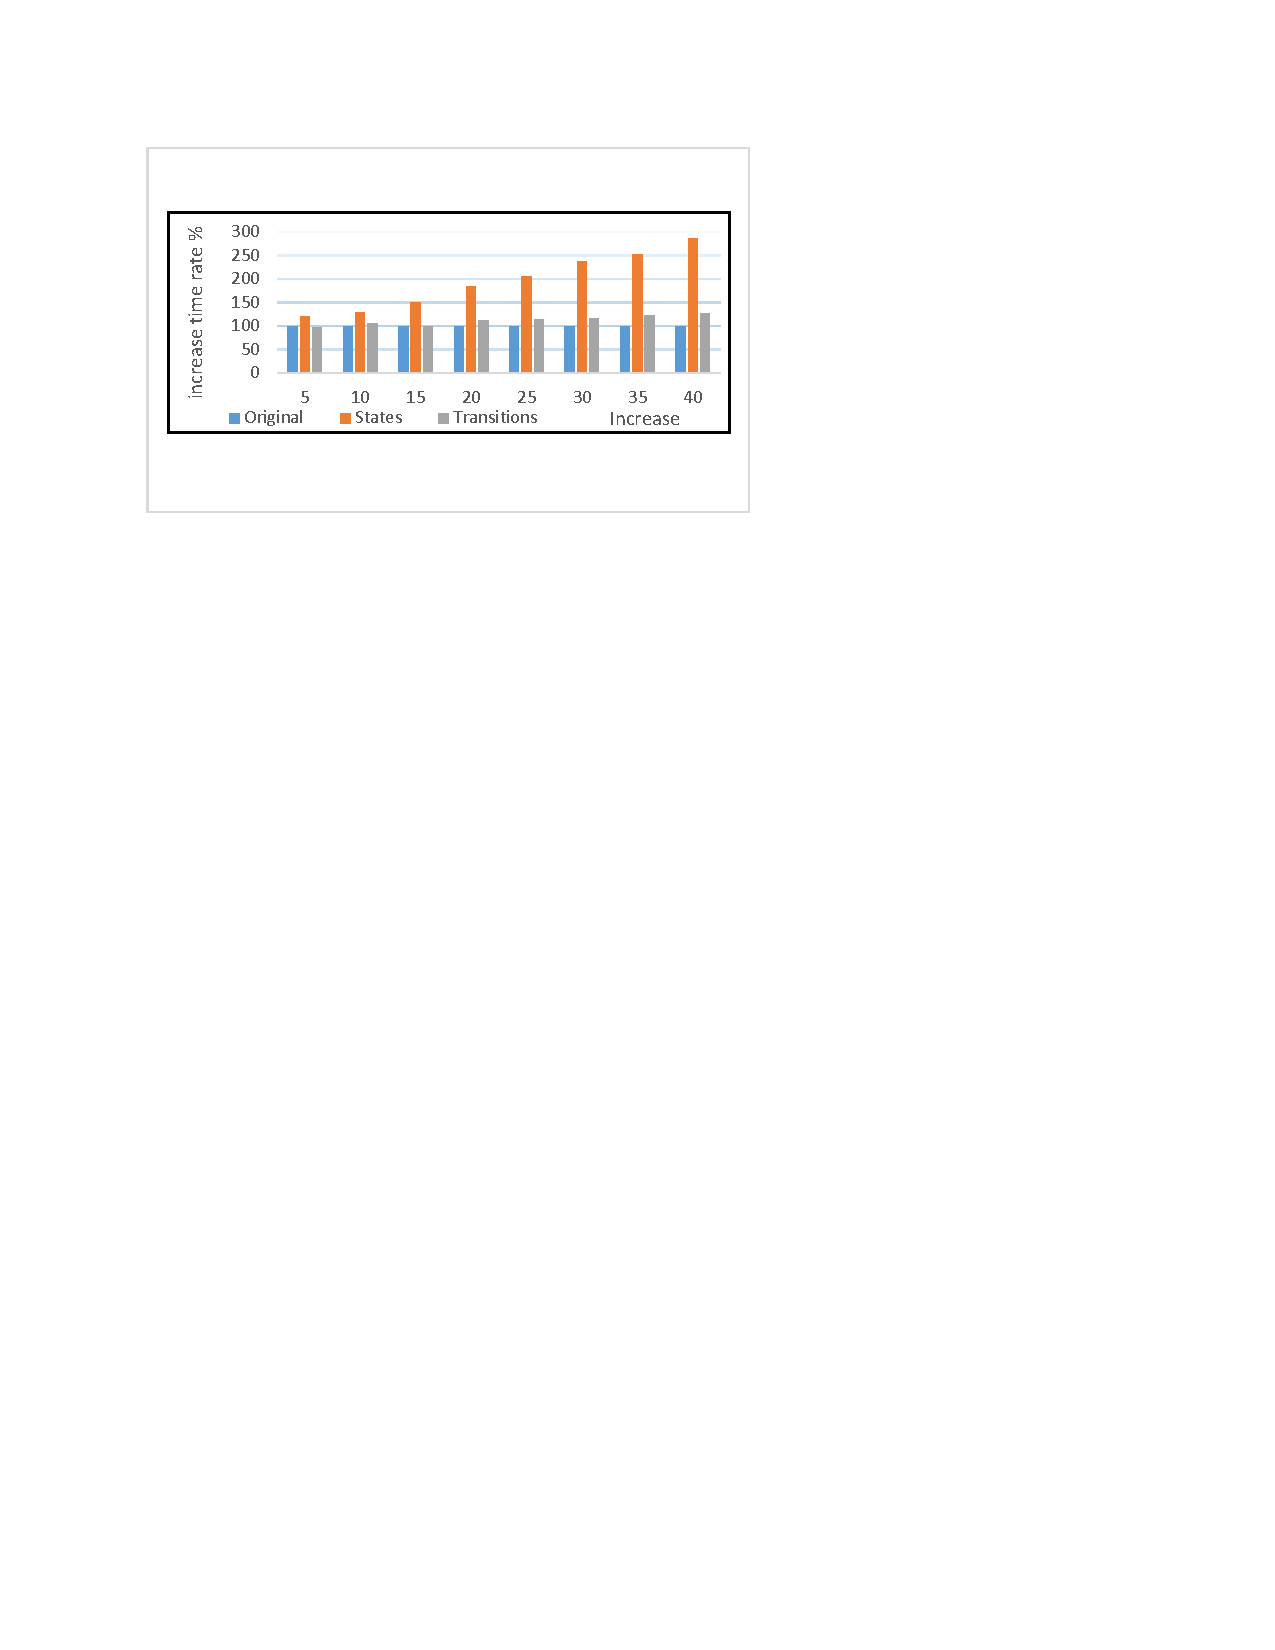
\includegraphics[clip, trim=2.8cm 20.6cm 9cm 3.6cm, width=0.35\textwidth]{figures/graph}
\caption{Performance impact comparison between states and transitions} 
\label{fig:graph}
\end{figure}

\subsection{Semantic conformance of runtime execution}
\label{subsec:exp2}
\paragraph{Bisimulation for semantic-conformance}
To evaluate the semantic conformance of runtime execution of generated code, we use a set of examples provided by Moka \cite{moka}. Moka is a model execution engine offering Precise Semantics of UML Composite Structures \cite{OMG2015}. Fig. \ref{fig:semanticconformance} shows our method. We first use our code generator to generate code (Step (1)) from the Moka example set. Step (2) simulates the examples by using Moka to extract the sequence (\ti{SimTraces}) of observed traces including executed actions. The sequence (\ti{RTTraces}) of traces is also obtained by the runtime execution of the code generated from the same state machine in a Step (3). The generated code is semantic-conformant if the sequences of traces are the same for both of the state machine and generated code \cite{Blech2005}. The current version of Moka does not support simulation for \ti{TimeEvent} and history pseudo states, we therefore leave experiments for \ti{TimeEvent} as future work.

For example, Fig. \ref{fig:autotransition} (a) shows a USM example with triggerless transitions (\ti{autotransitions}) \ti{T3}. 
The USM contains two states, \ti{Waiting}, which is the initial state, and \ti{Incrementing}, which increases an integer number from 0 to 5 by using the effect of \ti{T3}. The latter also has a guard checking whether the number is less than 5.
The increase is executed after the USM receives an event named \ti{start} to transition the initial state \ti{Waiting} to \ti{Incrementing}. 
Suppose that executions of the effects of \ti{T3} and \ti{T4} produce traces \ti{<T3>} and \ti{<T4>} (by using MOKA, e.g.), respectively. 
Due to the guard of \ti{T3}, the effect of \ti{T3} is executed five times followed by an execution of the effect of \ti{T4}.
After the completion of the USM, the obtained sequence of traces
is \ti{<T3><T3><T3><T3><T3><T4>}. 
The sequence obtained by the runtime execution of the code generated from this USM must be equivalent. 
\ti{RTTraces} is obtained by simply printing logging information for each action (effect).

Within our scope as previously defined 30 examples of the Moka example set are tested. \ti{SimTraces} and \ti{RTTraces} for each case are the same. 
This indicates that, within our study scope, the runtime execution of code generated by our generator can produce traces semantically equivalent to those obtained via simulation. 


After experimenting with our code generator, we compare our results to the observed traces obtained by executing code generated 
%by IBM Rhapsody \cite{ibm_rhapsody} and 
Umple \cite{Badreddin2014}. 
We find that the obtained traces in case of 
%IBM Rhapsody and 
Umple are not UML-compliant in triggerless transitions and some cases of event processing.
Specifically, for the example in Fig. \ref{fig:autotransition} (a), 
code generated by Umple only produces \ti{<T3>} as the trace sequence. 
Umple does not support events which are accepted by sub-states and the corresponding composite state as in Fig. \ref{fig:autotransition} (b) in which both \ti{S1} and \ti{S21} accept the event \ti{Continue}.
%Rhapsody does not support self-triggerless transitions as in Fig. \ref{fig:autotransition} and its support for processing events is not totally semantically correct. 
As the processing event example in Fig. \ref{fig:autotransition} (b), assuming that there is an event \ti{Continue} incoming to the state machine which has a current configuration \ti{(S1, S21)} as current active states. While, according to the UML specification, the incoming event should be processed by the inner states of the active composite/concurrent state if the inner states accept it, otherwise the parent state does. Therefore, the next configuration should be \ti{(S1, final state)} and the \ti{T22Effect} effect of the transition \ti{T22} should be executed. %But in case of Rhapsody the next configuration is \ti{End}.   


\begin{figure}
\centering
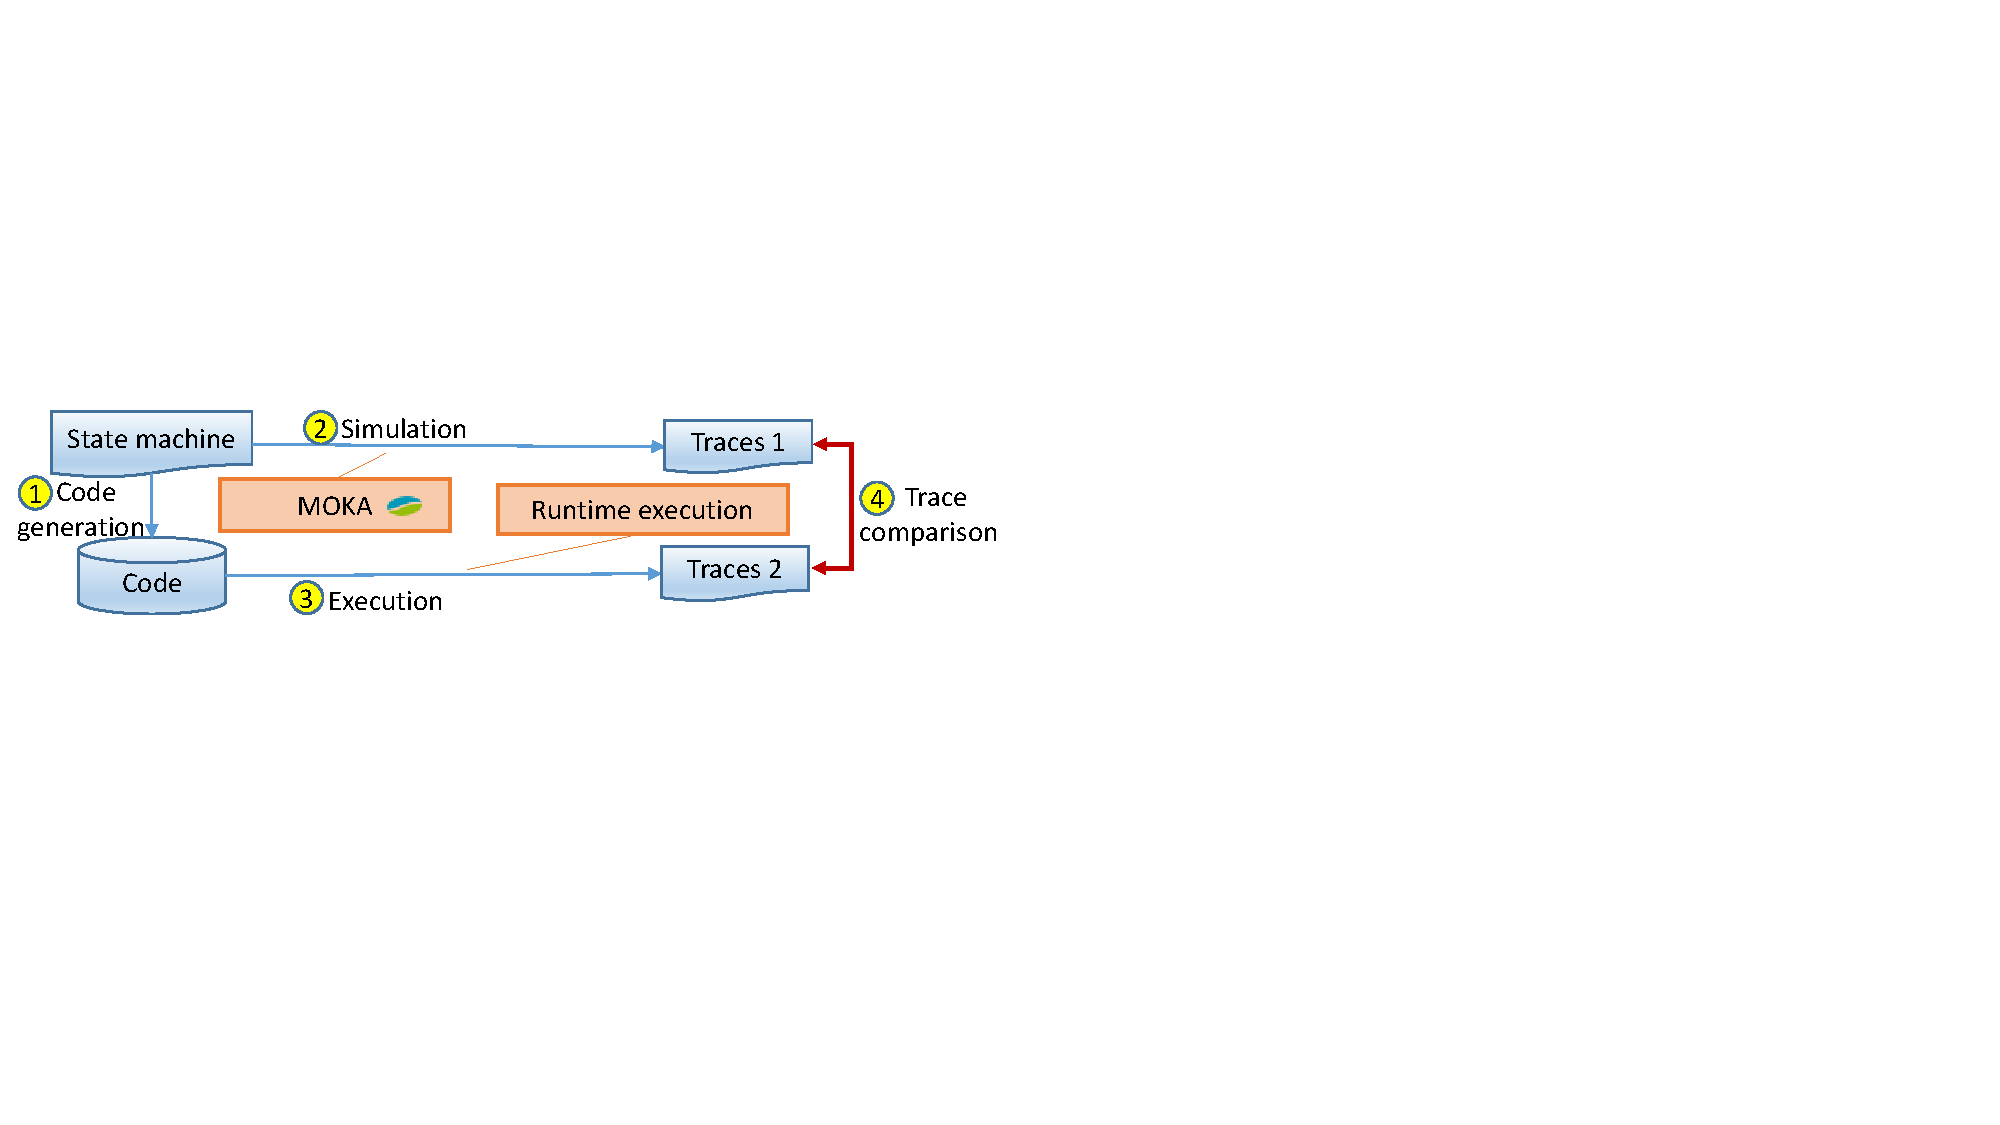
\includegraphics[clip, trim=0.2cm 8.6cm 19.4cm 6.9cm, width=0.8\columnwidth]{figures/semanticconformance.pdf}
\caption{Semantic conformance evaluation methodology} 
\label{fig:semanticconformance}
\end{figure}

\begin{figure}
\centering
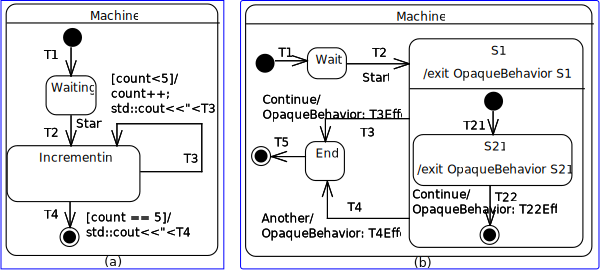
\includegraphics[clip, trim=0cm 0cm 0cm 0cm, width=\columnwidth]{figures/Deferred004Revised}
\caption{Self-triggerless transition and event processing example} 
\label{fig:autotransition}
\end{figure}



\begin{comment}
\begin{figure}
\centering
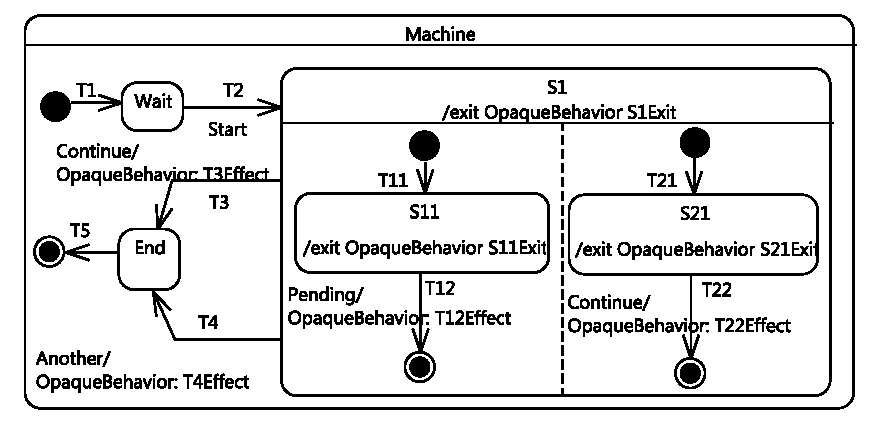
\includegraphics[clip, trim=0.25cm 0.25cm 0.25cm 0.25cm, width=0.9\columnwidth]{figures/Deferred004}
\caption{Event processing example} 
\label{fig:Deferred}
\end{figure}


\begin{figure*}
\centering
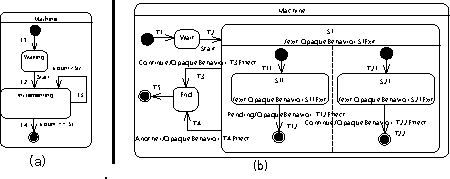
\includegraphics[width=1.5\columnwidth]{figures/ex}
\caption{Self-triggerless transition (a) and event processing (b) examples} 
\label{fig:ex}
\end{figure*}
\end{comment}

\paragraph{Finite state machine}
In addition to the experiment using MOKA, we evaluate the semantic-conformance by using deterministic finite state machines (FSMs). The latter is a mathematical model of computation and also a simplified version of UML state machine. In this experiment, we use FSMs for recognizing input symbols. Each FSM contains many atomic states. The active state of the FSM can be changed following the acceptance of an input symbol. Fig. \ref{fig:fsm} shows our method to experiment. For each FSM, we create an equivalent USM. Each input symbol of the FSM is considered as an event of the USM. We use the FSM simulator in \cite{fsmsim} to generate and simulate FSMs. For each FSM, a list of observed states is recorded as output (\ti{out1}) of the simulation for each symbol list. The latter is also the input of the generated code runtime execution of the equivalent USM which produces an output \ti{out2}. We then compare \ti{out1} and \ti{out2}.

We limit the number of FSMs to 20 and the number of symbol list for each FSM to 30 for practical concerns. 600 sequences of states obtained by the simulation and a same number of sequences taken by the runtime execution are respectively compared and found being equal. This results that our code generation approach can produce semantic-conformant code in case of FSM.

\begin{figure}
	\centering
	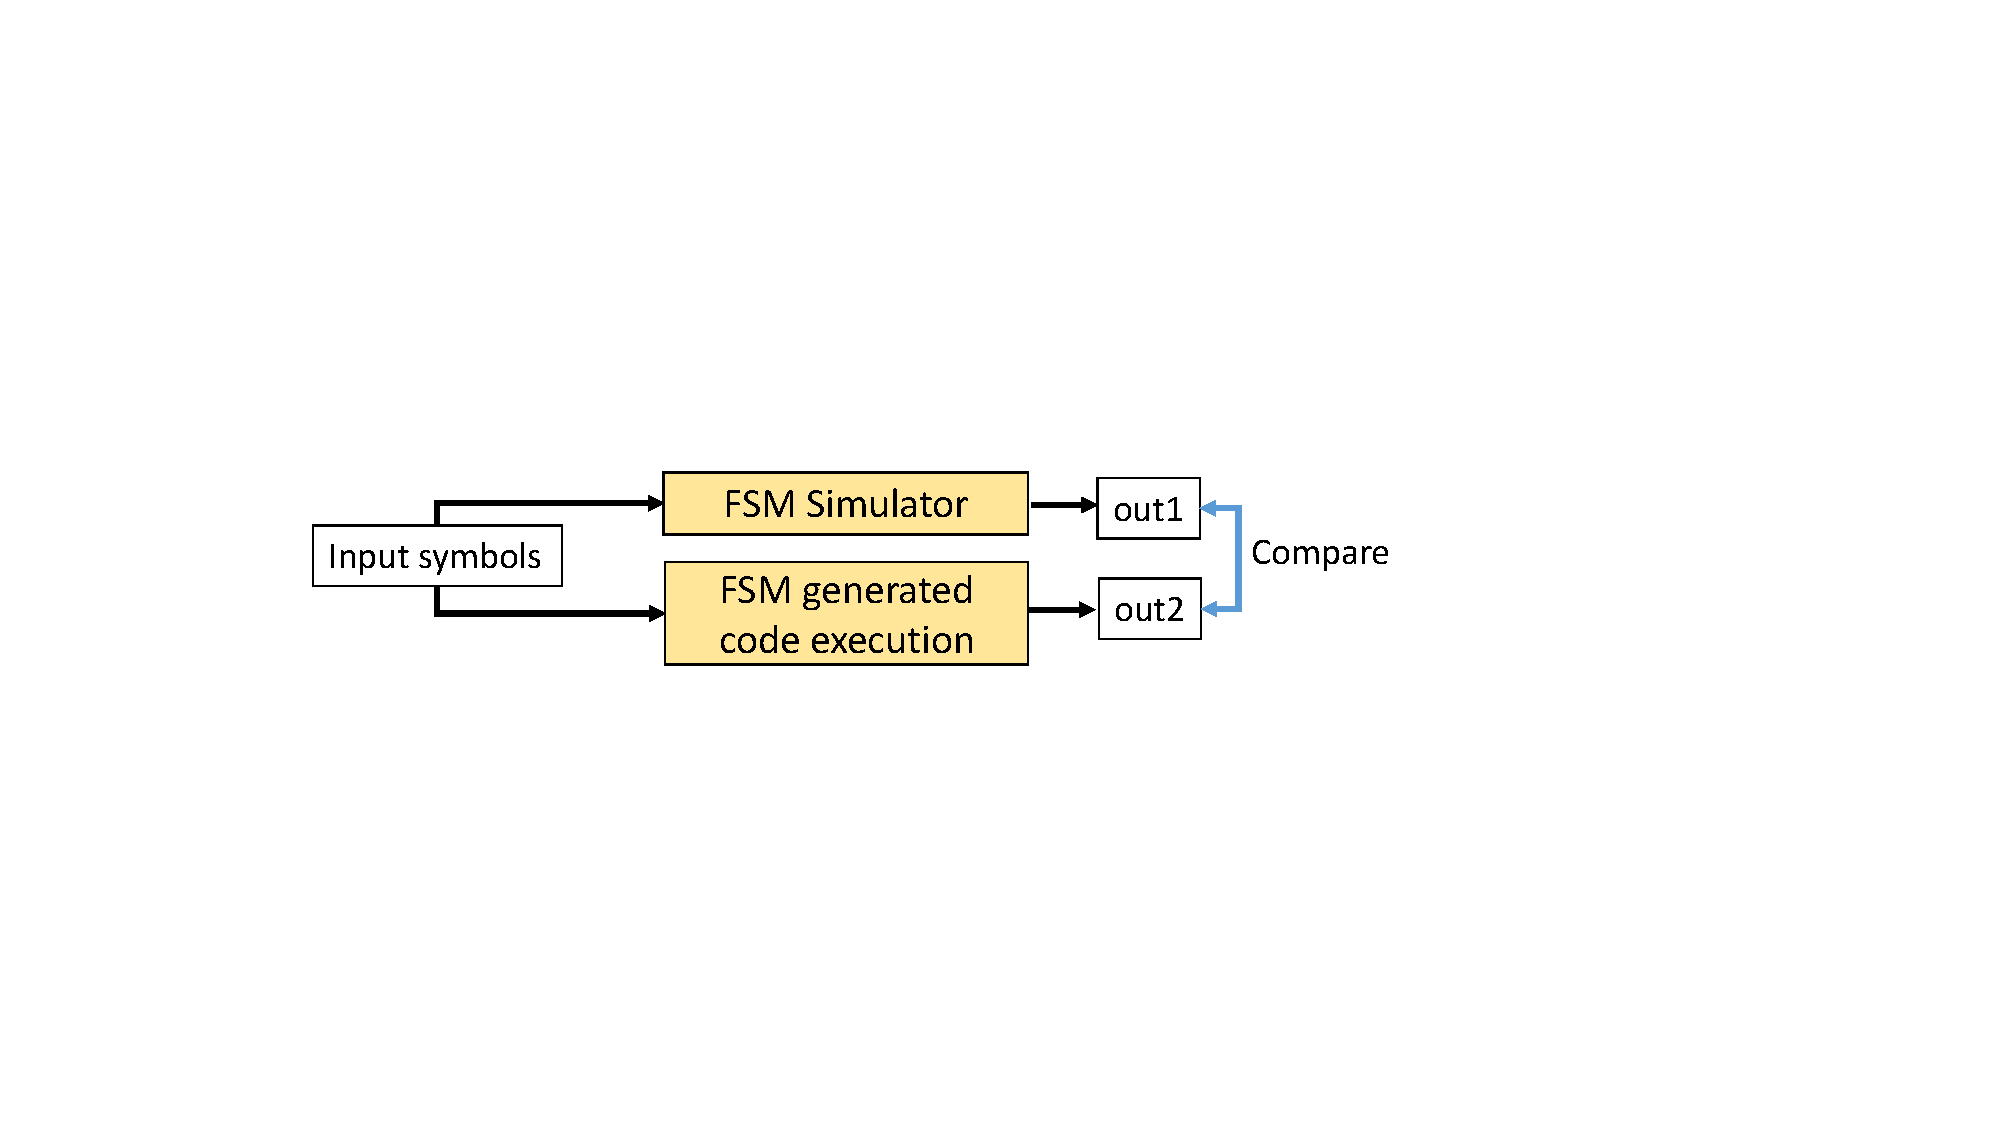
\includegraphics[clip, trim=4.5cm 7.6cm 10.25cm 8.0cm, width=0.85\columnwidth]{figures/fsm}
	\caption{FSM experiment method} 
	\label{fig:fsm}
\end{figure}

%\paragraph{Comparison with IBM Rhapsody}

\subsection{Development/maintenance cost}
\label{subsec:cost}
To compare the development/maintenance cost, we investigate steps need to be done in generated code and models, respectively, to do semantically equivalents. For example, to add a state, on one hand, one step needed in USM diagrams is \ti{dragging \& dropping the state notation to the appropriate parent}. On the other hand, three code modifications are (1) \ti{create a state class inheriting from the base state and its constructors}, (2) \ti{add to the parent state class an attribute}, and (3) \ti{add a line of code to initialize the state attribute in the parent state constructor}. Table \ref{table:cost} shows the number of steps needed for each operation. In this table, model manipulations are the winner in most of cases due to graphical representation advantages but code manipulations are still useful and comparable.

\begin{table}
\centering
\caption{Cost comparison}
\label{table:cost}
\begin{tabular}{|l|l|l|}
\hline
\rowcolor{Gray}
Description                                     & Model & Code \\ \hline
Add a state                                     & 1     & 3    \\ \hline
Add a transition                                & 1     & 3    \\ \hline
Add entry/exit action                           & 2     & 2    \\ \hline
Add transition action (effect) or guard                           & 2     & 2    \\ \hline
Update action/guard                                   & 1     & 1    \\ \hline
Redirect target state of a transition           & 1     & 1    \\ \hline
Create a call event to a transition & 3     & 6    \\ \hline
Create a time event to a transition & 3     & 5    \\ \hline
Delete a state                                  & 1     & 2    \\ \hline
Delete a transition                             & 1     & 3    \\ \hline
Delete entry/exit action                        & 1     & 2    \\ \hline
Delete transition action                        & 1     & 2    \\ \hline
Delete a call event                             & 2     & many \\ \hline
Delete a time event                             & 2     & many \\ \hline
\end{tabular}
\end{table}

In software development, programmers might modify the generated code, the modifications might violate structures of code or USM semantics. To resolve this issue, as previously described, we provide a semantic analysis that partly and loosely inspects the AST of generated code. This inspection approach always reverses the code to the USM as well as the code is state machine-compliant even though the code is not compiled. This approach is very useful in practice in which programmers might partly modify code, automatically update the original USM by our RTE, and automatically re-generate state machine-compliant code. This re-generation does no more than completing missing elements in code meaning that all previous changes are preserved. This practice is also limitedly supported by Fujaba \cite{KNNZ99_2_ag} in which activity and collaboration diagrams are partly synchronized with JAVA.




\section{Related Work}
\label{sec:related_works}
Our work is motivated by the desire to reduce the gap between and synchronize artifacts at different levels of abstraction, model and code in particular, in developing reactive systems. Specifically, the usage of USMs for describing the logical behavior of complex, reactive systems is indispensable. In the following sections, we compare our approach to related topics recorded in the literature.
\subsection{Implementation and code generation techniques for USMs}
Implementation and code generation techniques for USMs are closely related to the forward engineering of our RTE.
%Main approaches including switch/if, state table and state pattern are investigated.

%Switch/if is the most intuitive technique implementing a "flat" state machine. Two types of switch/if are supported. The first one uses a scalar variable representing the current active state \cite{Booch1998}. A method for each event processes the variable as a discriminator in switch/if statement. The second one uses a double nested switch/if and has two variables to represent the current active state and the event to be processed \cite{Douglass1999}. The latter are used as the discriminators of an outer switch statement to select between states and an inner one/if statement to decide how the event should be processed. The behavior code of the two types is put in one file or class. This practice makes code cumbersome, complex, difficult to read and less explicit when the number of states grows or the state machine is hierarchical. Furthermore, the first approach lets the code scatter in different places. Therefore, maintaining or modifying such code of complex systems is very difficult.

Switch/if is the most intuitive technique implementing a "flat" state machine. The latter can be implemented by either
using a scalar variable \cite{Booch1998} and a method for each event or using two variables as the current active state and the incoming event used as the discriminators of an outer switch statement to select between states and an inner one/if statement, respectively. The double dimensional state table approach \cite{Douglass1999} uses one dimension represents states and the other one all possible events. 
%Each cell of the table is associated with a function pointer meaning that the state associated with a dimension index of the cell is triggered by the event associated with the other dimension. 
The behavior code of these techniques is put in one file or class. This practice makes code cumbersome, complex, difficult to read and less explicit when the number of states grows or the state machine is hierarchical. 
%Therefore, maintaining or modifying such code of complex systems is very difficult. 
Furthermore, these approaches requires every transition must be triggered by at least an event. This is obviously only applied to a small sub-set of USMs.  
  
State pattern \cite{Shalyto2006,Douglass1999} is an object-oriented way to implement flat state machines. Each state is represented as a class and each event as a method. %The event is processed by a delegation from the context class to sub-states. 
Separation of states in classes makes the code more readable and maintainable. %Unfortunately, this technique only supports flat state machines. 
This pattern is extended in \cite{niaz_mapping_2004} to support hierarchical-concurrent USMs. However, the maintenance of the code generated by this approach is not trivial since it requires many small changes in different places. %This is impractical when dealing with large state machines. %Furthermore, similar to the state table, this approach also poses the requirement of having at least one event for transition.

Many tools, such as \cite{ibm_rhapsody, sparxsystems_enterprise_2014}, apply these approaches to generate code from USMs. Readers of this paper are recommended referring to \cite{Domnguez2012} for a systematic survey on different tools and approaches generating code from USMs.

Double-dispatch (DD) pattern in \cite{spinke_object-oriented_2013} in which %as a new technique to implement state machines. 
represent states and events as classes. Our generation approach relies on and extends this approach. The latter profits the polymorphism of object-oriented languages. %provides some 1-1 mappings from state machines to object-oriented code and the implementation technique 
%is not dependent on a specific programming language. 
However, DD does not deal with triggerless transitions and different event types supported by UML such as \ti{CallEvent}, \ti{TimeEvent} and \ti{SignalEvent}. Furthermore, DD is not a code generation approach but an approach to manually implementing state machines.

\subsection{Round-trip engineering}
Our RTE is related to synchronization of model-code and models themselves that a large number of approaches support. This paper only shows the most related approaches. 

\noindent
\ti{Model-code synchronization}

Commercial and open-source tools such as \cite{sparxsystems_enterprise_2014, ibm_rhapsody} only support RTE of architectural model elements and code.
Systematic reviews of some of these tools are available in \cite{Cutting2015}.

% RTE restriction
Some RTE techniques restrict the development artifact to avoid synchronization problems.
Partial RTE and protected regions \cite{Frankel:2002:MDA:579151} aim to preserve code changes which cannot be propagated to models.
This approach separates the code regions that are generated from models
from regions which are allowed to be edited by developers. 
This form of RTE is unidirectional only and does not support iterative development \cite{Jorges2013}
Our approach does not separate different regions but supports a semantic code analysis in the reverse direction.

Fujaba \cite{KNNZ99_2_ag} offers an RTE environment. An interesting part of Fujaba is that it abstracts from Java source code to UML class diagrams and a so-called story-diagrams. Java code can also be generated from these diagrams. RTE of these diagrams and code works but limited to the naming conventions and implementation concepts of Fujaba which are not UML-compliant. 

\noindent
\ti{Model synchronization}

RTE of models is tackled by many approaches categorized by its model transformation from total, injective, bi-directional to partial non-injective transformations \cite{Hettel2008}. %The authors in \cite{Paesschen2005} propose an injective mapping of elements in the source model to
%the target model. 
Techniques and technologies, such as Triple Graph Grammar (TGG) \cite{giese_incremental_2006}
and QVT-Relation \cite{Omg2008},
allow synchronization between source and target elements that have non-injective mappings.
These techniques require a mapping model to connect the source and target models which need to be persisted in a model store \cite{Bergmann2011}.
Mappings between USMs and code in our approach are non-bijective. We only use simple tables for storing tracing information.

%Foster et al \cite{foster_combinators_2007} uses the concepts of lenses to define RTE. A lens consists of a \ti{get} function, which produces a target artifact (model/code) from a source artifact (model/code), and a \ti{putback} function, which takes as input the modified target and old source artifact to update the source artifact. The paper also defines two RTE laws that a RTE must satisfy. These laws are the base for the evaluation of our approach that will be presented in Section \ref{sec:experiments}.  
 

%\ti{Partial RTE} and \ti{protected regions} are introduced in \cite{Frankel:2002:MDA:579151} and \cite{Kelly2007} to preserve code modifications which cannot be reflected to models. This approach separates the code part which is generated from models and the part which is allowed to be changed by programmers. This form of RTE is unidirectional only and does not support iterative development \cite{Jorges2013}. 

%RTE of UML models and object-oriented code are supported in many tools including research prototypes and commercial such as Enterprise Architect \cite{sparxsystems_enterprise_2014}, Visual Paradigm \cite{visual}, AndroMDA \cite{_andromda_}. Although these tools work well with UML class diagrams and code, behavioral diagrams are not well supported.  

%The authors in \cite{angyal_synchronizing_2008} propose a syntactic synchronization technique for domain-specific modeling languages (DSML) and code. The approach uses an Abstract Syntax Tree (AST) metal-model to model source. Changes in code detected by using an algorithm proposed  in \cite{Chawathe:1996:CDH:235968.233366}. %to compare the AST instance of the current code with the last synchronized one are merged to the instance of DSML. 
%However, an AST is very low level and it is not clear to have mappings from DSML instances to AST instances. Furthermore, although there is an example for illustrating the technique, a systematic evaluation of the approach is not presented to show its scalability.


%Other techniques \cite{foster_combinators_2007}
%are based on bi-directional transformations, which comprise a forward transformation a backward transformation.
%Bi-directional transformations provides a novel mechanism for synchronization.
%Some works \cite{Matsuda2015} derive a backward transformation based on forward
%transformation.
%However, such works do not offer any means to synchronize models that are concurrently edited.

%A few approaches derive model synchronization from model transformation while allowing concurrent editions
%of both source and target models.
%In \cite{xiong_towards_2007} the authors propose to automatically derive
%model synchronization of a source and a target model related by an ATL \cite{eclipse_foundation_eclipse_2016}
%model transformation.
%The synchronization is based on differentiating source and target model states.
%But, reflectable addition of an element in the target model is not well handled according to \cite{xiong_towards_2007}.
Differently from other approaches, ours is specific to RTE of USMs and code. The goal is to provide a full model-code synchronization supporting for rapidly, iteratively, and efficiently developing reactive systems. 
\section{Conclusion}


%\section*{Appendix}
%Appendixes, if needed, appear before the acknowledgment.

\section*{Acknowledgment}
The work presented in this paper is supported by the European project SafeAdapt, grant agreement No. 608945, see \ti{http://www.SafeAdapt.eu}. The project deals with adaptive system with additional safety and real time constraints. The adaptation and safety aspects are stored in different artifacts in order to achieve a separation of concerns. These artifacts need to be synchronized.


\balance
\bibliographystyle{IEEEtran}
\bibliography{refs}



\end{document}
